\section{Lecture 11: Sample and Hold}

\subsection{Introduction}
In the last session we have seen that sampling is actually multiplying an input signal with a periodic waveform. Sampling is about representing the signal more efficiently than the raw form. 
In this discussion we discuss the problem of reconstruction of the signal if we put in place systems to interpolate the signal from the sampled signal.
%about what we want to do with the sampled signal, i.e. whether we want to hold on to the sampled signal or just let it go. 

\subsection{Interpolation}
Interpolate means to complete the waveform in between the samples. Interpolation is a method of constructing new data points within the range of a discrete set of known data points.

\subsubsection{Graphical Explanation}

Let us consider a function as shown in fig. 1 and sample it with a time period of $T_{s}$.

\begin{figure}[ht]
\centering
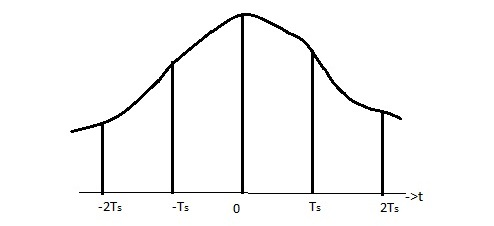
\includegraphics[width=0.6\textwidth]{M3L11-fig1.jpg}
\caption{A sampled function}
\end{figure}

There are various ways in which we can interpolate the given samples\\


\noindent Method 1: Sample and Hold\\
\noindent In figure 2, the red lines form the interpolated signal using the Sample and Hold method.

\begin{figure}[ht]
\centering
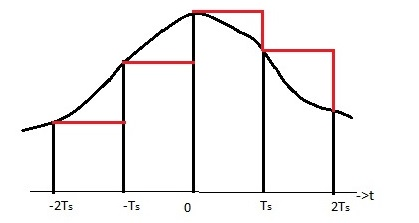
\includegraphics[width=0.6\textwidth]{M3L11-fig2.jpg}
\caption{Sample and Hold}
\end{figure}


\noindent Method 2: Linear interpolation\\
In this method the sampled points are connected by straight lines. Refer to figure 3 for linear interpolation.
In Figure 3, the green lines form the linearly interpolated signal obtained by interpolating from the sampled signal.



\begin{figure}[ht]
\centering
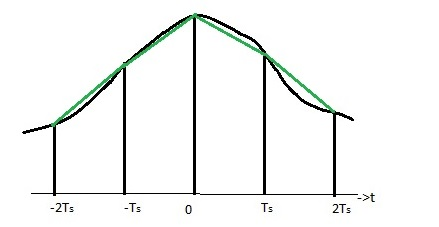
\includegraphics[width=0.6\textwidth]{M3L11-Fig3.jpg}
\caption{Linear interpolation}
\end{figure}


Other kinds of interpolations are also possible. But in this discussion we shall focus on sample and hold.

\subsubsection{Systematical explanation}

Systematically the sample and hold can be understood as follows:

\begin{figure}[ht]
\centering
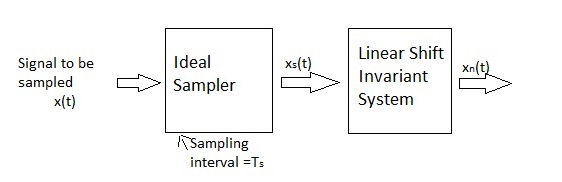
\includegraphics[width=0.7\textwidth]{M3L11-fig4.jpg}
\caption{Systematical representation of sample and hold}
\end{figure}

The impulse response of the linear shift invariant system in the above figure is a pulse as shown in fig 5.

\begin{figure}[ht]
\centering
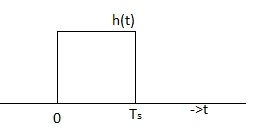
\includegraphics[width=0.5\textwidth]{M3L11-Fig5.jpg}
\caption{Impulse response of linear shift invariant system.
}\end{figure}

\subsection{Frequency domain analysis}
The LSI system which follows the ideal sampler is called the Hold system. This is because, the effect of this system on a sampled signal is that of retaining the sampled value till the next sample is reached. Note that since the Hold system impulse response has a finite value in a finite interval, it is absolutely integrable and hence it is a stable system.
%The hold system can be stated to be stable as the impulse response is absolutely integrable. 
\\
Now, the frequency response of the Hold system is:

\begin{align*}
H(\Omega) &=\int\limits_{-\infty}^{\infty}\mathrm{h(t)}{e}^{-jt\Omega}\,\mathrm{d}\\
&=\int\limits_{0}^{T_{s}}\mathrm{e}^{-jt\Omega}\,\mathrm{d}t\\
&=\left.\frac{e^{-jt\Omega}}{-j\Omega}\right|_0^{T_{s}}\\
&=\frac{1-e ^{-j\Omega T_s}}{j \Omega}\\
&=\frac{e^\frac{-j \Omega T_s}{2} \left(e^{\frac{j \Omega T_s}{2}} - e^{\frac{-j \Omega T_s}{2}}\right)}{j \Omega}\\
&=\frac{T_s}{2} e^{\frac{-j \Omega T_s}{2}} \frac{2j \sin{\frac{\Omega T_s}{2}}}{j \frac{\Omega T_s}{2}}\\
&=T_s e^\frac{-j \Omega T_s}{2}\frac{2j}{2j} \frac{\sin{\frac{\Omega T_s}{2}}}{\frac{\Omega T_s}{2}}\\
&=T_s e^{\frac{-j \Omega T_s}{2}} \frac{\sin{\Omega T_s/2}}{\Omega T_s/2}
\end{align*}

%$$= \int\limits_{-\infty}^{\infty}\mathrm{h(t)}{e}^{-jt\Omega}\,\mathrm{d}t$$

%$$= \int\limits_{0}^{T_{s}}\mathrm{e}^{-jt\Omega}\,\mathrm{d}t$$
%$$= \left.\frac{e^{-jt\Omega}}{-j\Omega}\right|_0^{T_{s}}=\frac{1-e ^{-j\Omega T_s}}{j \Omega}$$


%$$= \frac{e^\frac{-j \Omega T_s}{2} \left(e^{\frac{j \Omega T_s}{2}} - e^{\frac{-j \Omega T_s}{2}}\right)}{j \Omega}$$
%$$=\frac{T_s}{2} e^{\frac{-j \Omega T_s}{2}} \frac{2j sin{\frac{\Omega T_s}{2}}}{j \frac{\Omega T_s}{2}}$$
%$$=T_s e^\frac{-j \Omega T_s}{2}\frac{2j}{2j} \frac{sin{\frac{\Omega T_s}{2}}}{\frac{\Omega T_s}{2}}$$
%Frequency response
%{\Large
% = $T_s e^{\frac{-j \Omega T_s}{2}} \frac{sin{\Omega T_s/2}}{\Omega T_s/2}$
%}

\subsubsection{Frequency domain analysis}

Let $x(t)$ obey Nyquist principle. Hence band limited to $\frac{1}{2 T_s}$.
Consider such an $x(t)$ with Fourier Transform as shown in Figure 6.
%\noindent If $x(t)$ is band limited, the Fourier transform in ycles/second is as follows:

\begin{figure}[ht]
\centering
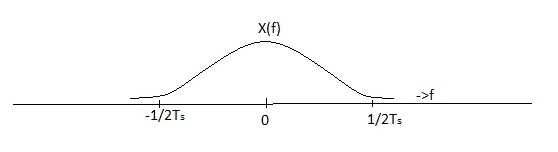
\includegraphics[width=0.9\textwidth]{M3L11-fig6.jpg}
\caption{Fourier transform of x(t)}
\end{figure}

Then, after passing the signal through the ideal sampler, the sampled signal obtained, $X_s(t)$, will have the spectrum $X_s(f)$ as shown in Figure 7.


\begin{figure}[ht]
\centering
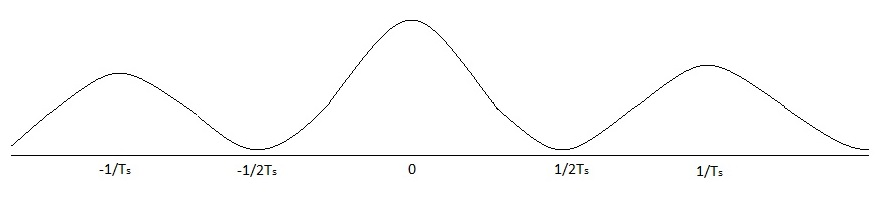
\includegraphics[width=0.9\textwidth]{M3L11-Fig7.jpg}
\caption{Spectrum of the sampled signal: $X_{S}(f)$}
\end{figure}

Sketch of 'hold' frequency response.

$$ H(f) = T_s e^{-j \pi fT_s}\frac{sin \pi fT_s}{\pi fT_s}$$

Magnitude $\implies$

\begin{figure}[ht]
\centering
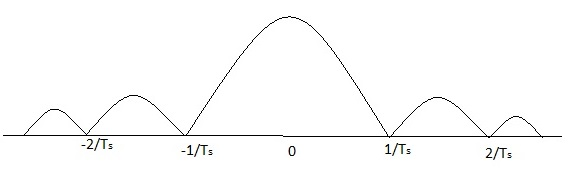
\includegraphics[width=0.9\textwidth]{M3L11-Fig8.jpg}
\caption{Hold frequency response}
\end{figure}

If we superimpose both hold frequency response and $X_s(f)$,

\begin{figure}[ht]
\centering
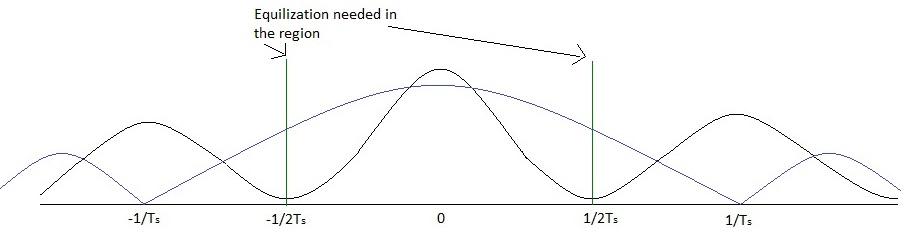
\includegraphics[width=1.2\textwidth]{M3L11-Fig9.jpg}
\caption{Superimposing hold freq. response on $X_{s}(f)$}
\end{figure}


In process of sampling and holding, two problems are
\begin{enumerate}
\item Aliases pass through partially
\item Original gets distorted
\end{enumerate}


Hence, equalization is needed in the original spectral band of

$-\frac{1}{2T_s} \rightarrow \frac{1}{2T_s}$

Equalization is the reciprocal of the hold frequency response given by\\
{\large
$$\frac{1}{T_s e^{-j \pi f T_s}\frac{\sin \pi fT_s}{\pi f T_s}}
\mbox{  for} -\frac{1}{2T_s} < f <  \frac{1}{2 T_s}$$
}
\newpage

Sketch of equalizer frequency response.

\begin{figure}[ht]
\centering
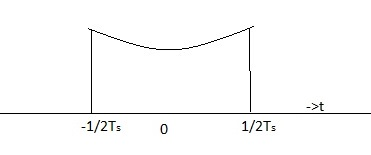
\includegraphics[width=0.7\textwidth]{M3L11-Fig_10.jpg}
\caption{Equalizer freq. response}
\end{figure}


Hence to reconstruct a signal after sample and hold, two things are required:
\begin{enumerate}
\item To remove the aliases
\item To equalize
\end{enumerate}

The ideal reconstructor for sample and hold has to
\begin{enumerate}
\item Equalize in signal band
\item Stopband outside sigal band
\end{enumerate}

In the next lecture, we will discuss about linear interpolation.

